\documentclass{beamer}
\usepackage[ngerman]{babel}
\usepackage[utf8]{inputenc}
\usepackage{graphicx}
\usepackage{hyperref}
\graphicspath{{./assets/}}

\title{Modern Algorithms for Garbage Collection}
\subtitle{Outlining modern algorithms for garbage collection on the examples of Go and Java}
\date[2023]{2023}
\author{9525469, 6424019} 

\institute[DHBW Mosbach]{DHBW Mosbach}

\date{\today}

\usetheme{metropolis}
\setbeamertemplate{navigation symbols}{}
\setbeamertemplate{footline}[frame number]

\begin{document}
    
    \frame{\titlepage}

    \tableofcontents
    
	\section{Garbage collection}
        \begin{frame}
            \frametitle{Garbage collection}

            Garbage collection ist definiert als

            \begin{itemize}
                \item Erkennung von nicht mehr verwendeten Speicherbereichen
                \item automatisches Entfernen von nicht mehr verwendeten Speicherbereichen
            \end{itemize}

            Und zielt darauf ab das obige:

            \begin{itemize}
                \item schnell
                \item effizient
                \item mit wenig Latenz
                \item mit wenig RAM und CPU Auslastung
            \end{itemize}

            umzusetzen.
        \end{frame}

        \subsection{Garbage collection - Nutzen}
            \begin{frame}
                \frametitle{Garbage collection - Nutzen}

                Befreit den Programmierer zumeist von:
                \begin{itemize}
                    \item Manueller Speicherallokierung mit \texttt{malloc}, \texttt{calloc} und \texttt{realloc}
                    \item Manueller Speicherfreigabe mit \texttt{free}
                    \item Pointer arithmetik
                \end{itemize}

                Verhindert Fehler wie: \footnote{70\% der CVE's von Chromium sind Speicherzugriffbezogen, siehe: \href{https://www.chromium.org/Home/chromium-security/memory-safety/}{https://www.chromium.org/Home/chromium-security/memory-safety/}}
                \begin{itemize}
                    \item Seg faults (illegaler Speicherzugriff) 
                    \item Use after \texttt{free} (Speicherzugriff auf bereits aufgeräumte Speicherbereiche)
                    \item Memory leaks (Speicher wird nach Verwendung nicht freigegeben)
                \end{itemize}
            \end{frame}

        \subsection{Garbage collection - Problematiken}
            \begin{frame}
                \frametitle{Garbage collection - Problematiken}
                \begin{itemize}
                    \item Peformance schlechter im Vergleich zu manuellem
                        management und borrow checker
                        \begin{itemize}
                            \item Latenz 
                            \item RAM und CPU Verbrauch
                            \item Generational, Mark \& Sweep: Scannen vom Heap langsam
                            \item Reference counting: erhöhter Speicherverbrauch: 100 Objekte: $100*objektgroeße$ auf $100*(objektgroeße+countergroeße)$
                        \end{itemize}
                    \item Einfluss von GC-zyklen auf Program nicht vorhersehbar
                    \item Manuelle Allokationen mit Speicherarena effizienter
                        für große Datenmengen als jedes Objekt einzeln
                        allokieren
                \end{itemize}
            \end{frame}

    \section{Strategien}
        \begin{frame}
            \frametitle{Strategien}

            Strategien unterscheiden sich in ihrer:

            \begin{itemize}
                \item Erkennung von unerreichbaren Objekten
                \item Entfernung von unerreichbaren Objekten
                \item Latenz, RAM und CPU Verbrauch
            \end{itemize}
        \end{frame}

        \subsection{Mark \& Sweep}
            \begin{frame}
                \frametitle{Strategien - Mark \& Sweep}
            \end{frame}

        \subsection{Generational garbage collection}
            \begin{frame}
                \frametitle{Strategien - Generational garbage collection}
                Optimierung basierend auf der Beobachtung, dass die meisten Objekte nur kurzlebig sind (Infant Mortality)\\
                Aufteilung in drei Speicherbereiche aufgeteilt:
                \begin{itemize}
                    \item Young, bestehend aus Eden und Survivor Space
                    \item Old
                    \item Permanent
                \end{itemize}
                % Unterteilung des Heaps in die Generationen:
                % https://www.oracle.com/technetwork/tutorials/tutorials-1876574.html
                % https://www.oracle.com/webfolder/technetwork/tutorials/obe/java/G1GettingStarted/images/HeapStructure.png
                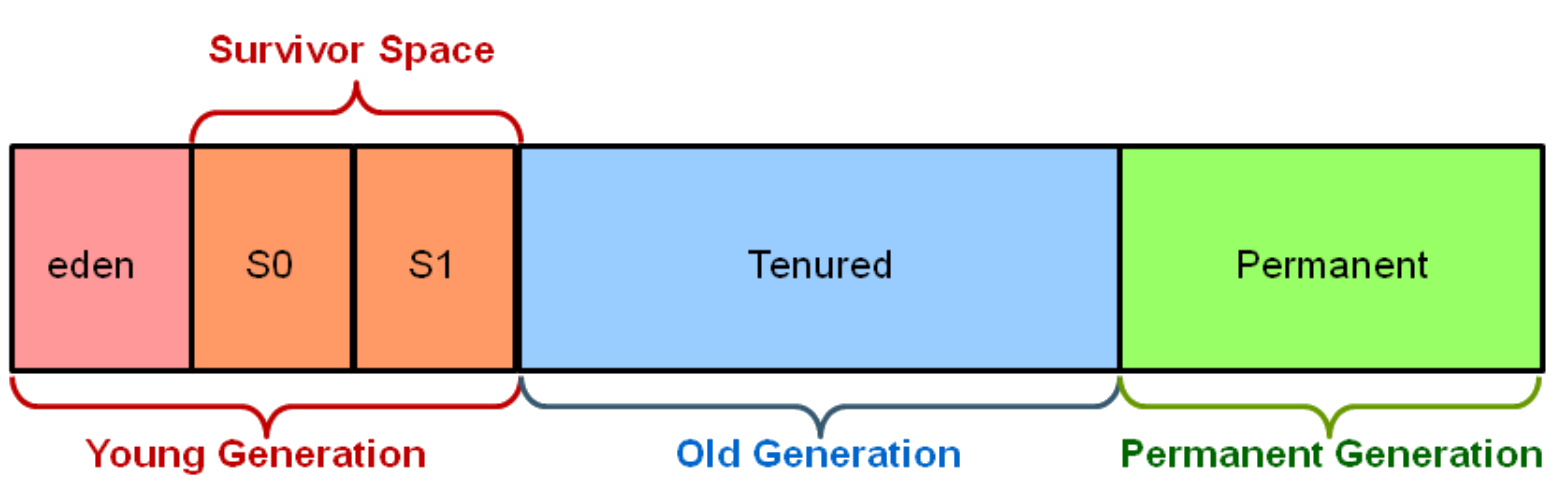
\includegraphics[width=\textwidth]{images/GenerationalGCHeapStructure.png}
            \end{frame}

            \begin{frame}
                \frametitle{Strategien - Generational garbage collection}
                \begin{itemize}
                    \item Eden
                    \begin{itemize}
                        \item Alle neuen Objekte werden hier allokiert
                        \item Objekte welche eine gewisse Zeit überleben werden in den Survivor Space verschoben
                    \end{itemize}
                    \item Survivor
                    \begin{itemize}
                        \item Hier sind Objekte welche eine gewisse Zeit überlebt haben
                        \item Objekte welche eine längere Zeit überlebt haben werden in den Old Space verschoben
                    \end{itemize}
                    \item Old
                    \begin{itemize}
                        \item Hier sind Objekte welche schon länger existieren und es unwahrscheinlich ist, dass sie bald gelöscht werden
                    \end{itemize}
                \end{itemize}
                Eden wird aufgrund von Infant Mortality häufig collected, ist aber klein da lang lebende Objekte nicht dort sind.
            \end{frame}

        \subsection{Reference counting}
            \begin{frame}
                \frametitle{Strategien - Reference counting}

                \begin{itemize}
                    \item Jedes Objekt hat einen Zähler, welcher die Anzahl der Referenzen auf das Objekt zählt.\\
                    \item Beim Erstellen eines Pointers auf das Objekt wird der Zähler inkrementiert, beim Löschen dekrementiert.\\
                    \item Wird der Zähler 0, so wird das Objekt deallokiert.
                \end{itemize}
                Probleme bei Referenzzyklen: Zähler wird nie 0, Objekte werden nicht gelöscht.
            \end{frame}

    \section{Programmiersprachen}
        \begin{frame}
            \frametitle{Programmiersprachen}

            \begin{itemize}
                \item Viele Sprachen mit und ohne GC
                \item Algorithmen, Implementierungen und Performance sehr unterschiedlich
                \item High level sprachen eher mit GC, low level eher ohne
            \end{itemize}
        \end{frame}

        \subsection{Ohne Garbage collection}
            \begin{frame}
                \frametitle{Programmiersprachen - Ohne gc}

                \begin{itemize}
                    \item C
                    \begin{itemize}
                        \item manuelles memory managment
                    \end{itemize}
                    \item C++
                    \begin{itemize}
                        \item manuelles memory managment
                        \item reference counting on demand
                    \end{itemize}
                    \item Rust
                    \begin{itemize}
                        \item borrow checker
                        \item reference counting on demand
                    \end{itemize}
                \end{itemize}
            \end{frame}

        \subsection{Mit Garbage collection}
            \begin{frame}
                \frametitle{Programmiersprachen - Mit gc}
                \begin{itemize}
                    \item Go
                    \begin{itemize}
                        \item escape analysis
                        \item mark \& sweep
                    \end{itemize}
                    \item Java
                    \begin{itemize}
                        \item mehrere garbage collectoren
                        \item generational standardmäßig
                        \item Compiliert in Bytecode(AOT), Ausführung mit Bytecode vm (JVM)
                    \end{itemize}
                    \item Python
                    \begin{itemize}
                        \item Reference counting
                        \item Erkennung von Referenzzyklen
                    \end{itemize}
                    \item JavaScript
                    \begin{itemize}
                        \item generational
                        \item JIT, Bytecode vm (V8)
                    \end{itemize}
                \end{itemize}
            \end{frame}

    \section{Implementierungen}
        \begin{frame}
            \frametitle{Garbage collection Implementierungen}
        \end{frame}

        \subsection{Go}
            \begin{frame}
                \frametitle{Implementierungen - Go}
            \end{frame}

        \subsection{Java}
            \begin{frame}
                \frametitle{Implementierungen - Java}
            \end{frame}

    \section{Performance}
        \begin{frame}
            \frametitle{Performance}

            Diverse Kriterien möglich, hier beschränkt auf:

            \begin{itemize}
                \item Speicherverbrauch: stärke RAM-Intensivität
                \item Latenz: Umfang Stoppzeiten des Programs
                \item Sicherheit: Speicherzugriffsicherheit
                \item Nutzbarkeit: Komplexität der Strategien
            \end{itemize}
        \end{frame}

        \subsection{Speicherverbrauch}
            \begin{frame}
                \frametitle{Performance - Speicherverbrauch}
            \end{frame}

        \subsection{Latenz}
            \begin{frame}
                \frametitle{Performance - Latenz}
            \end{frame}

        \subsection{Sicherheit}
            \begin{frame}
                \frametitle{Performance - Sicherheit}
            \end{frame}

        \subsection{Nutzbarkeit}
            \begin{frame}
                \frametitle{Performance - Nutzbarkeit}
            \end{frame}

\end{document}

